\begin{figure}[ht!]
  \center
  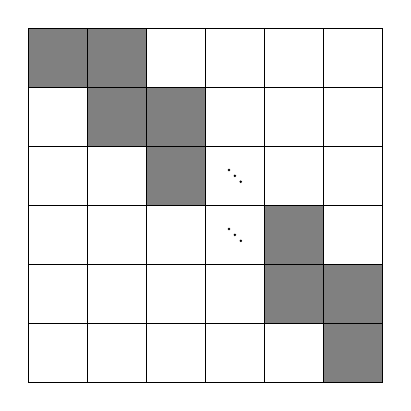
\begin{tikzpicture}[scale=0.75]
    \foreach \i/\j in {1/5, 2/5, 2/4, 3/4, 3/3, 5/2, 5/1, 6/1, 6/0} { \fill[gray] (\i, \j) rectangle (\i + 1, \j + 1); }
    \draw
      (4.4,3.6) circle (0.01)
      (4.5,3.5) circle (0.01)
      (4.6,3.4) circle (0.01)

      (4.4,2.6) circle (0.01)
      (4.5,2.5) circle (0.01)
      (4.6,2.4) circle (0.01)
    ;
    \draw (1,0) grid (7,6);
  \end{tikzpicture}
  ~
  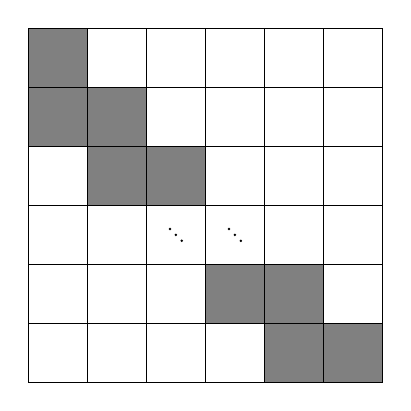
\begin{tikzpicture}[scale=0.75]
    \foreach \i/\j in {1/5, 1/4, 2/4, 2/3, 3/3, 4/1, 5/1, 5/0, 6/0} { \fill[gray] (\i, \j) rectangle (\i + 1, \j + 1); }
    \draw
      (3.4,2.6) circle (0.01)
      (3.5,2.5) circle (0.01)
      (3.6,2.4) circle (0.01)

      (4.4,2.6) circle (0.01)
      (4.5,2.5) circle (0.01)
      (4.6,2.4) circle (0.01)
    ;
    \draw (1,0) grid (7,6);
  \end{tikzpicture}
  ~
  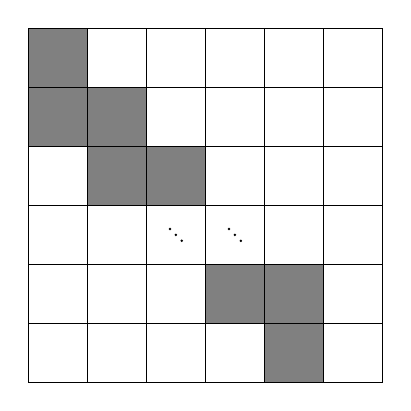
\begin{tikzpicture}[scale=0.75]
    \foreach \i/\j in {1/4, 1/5, 2/3, 2/4, 3/3, 4/1, 5/0, 5/1} { \fill[gray] (\i, \j) rectangle (\i + 1, \j + 1); }
    \draw
      (3.4,2.6) circle (0.01)
      (3.5,2.5) circle (0.01)
      (3.6,2.4) circle (0.01)

      (4.4,2.6) circle (0.01)
      (4.5,2.5) circle (0.01)
      (4.6,2.4) circle (0.01)
    ;
    \draw (1,0) grid (7,6);
  \end{tikzpicture}
  \caption{
    Three $n \times n$ blocks, two with $2n - 1$ crossed-out cells and one with $2n - 2$ crossed-out cells.
  }
  \label{fig:blockShape}
\end{figure}
